%advantages / disadvantages
Magnitude analysis is well-suited for answering research questions about the use of a single IDE command. However, many research questions are related to a specific part or tool in the IDE, which usually corresponds to multiple IDE commands. For instance, the research question ``How often are refactorings performed?'' cannot be answered via magnitude analysis alone, as refactorings can be triggered through a number of different IDE commands. These commands first need to be categorized, after which magnitude analysis can be used. 

When focusing on a concrete sub-task, such as refactoring, it may be easy to categorize activities. In this case, all refactoring commands, such as pull-up or extract method, can be classified as refactorings. However, when focusing on more general behavior, such as editing, navigating, and searching, categorizations can be difficult. It is impossible to say, for instance, from a single click in the File Explorer window, whether that click represents a search, as the developers browses a few promising files, or a navigation, as he implicitly opens a type declaration of a variable he was just browsing. Thus, categorization without context can produce noisy data in certain cases. However, caterigorization is a powerful tool, especially when there is little ambiguity in the IDE commands that are analyzed.

%example
Consider the research question ``Are developers successful in finding relevant program elements?'' and the following stream of IDE commands generated from a user's interaction with the Find-in-Files search tool, which is available in Visual Studio. We consider a developer to have been successful in finding relevant program elements if he or she performed one of the following actions after clicking on a search result: editing or following structural dependencies.

\begin{verbatim}
Collector Started
2014-02-02 13:46:52 - User submitted query to Find-in-Files
2014-02-02 13:46:56 - Find-in-Files retreived 121 results
2014-02-02 13:52:21 - User clicked on result 2
2014-02-02 13:58:01 - User clicked on result 8
2014-02-02 13:59:57 - Open caller/callee command 
...
2014-02-02 14:46:52 - User submitted query to Find-in-Files
2014-02-02 14:46:56 - Find-in-Files retreived 19 results
2014-02-02 15:01:08 - User clicked on result 11
2014-02-02 15:07:12 - Open definition command
Collector Stopped
\end{verbatim}

Following structural dependencies can be performed in several ways, two of which are the Open Caller/Callee command, which displays a list of methods that call and are called by the current method, and the Open Definition command, which opens the definition of a type. Categorization analysis would first determine each of the ways that following structural dependencies can be performed in the IDE and subsequently count these events, perhaps after a
Find-in-Files query was submitted as in the above listing, and calculate relevant metrics to answer the research questions. The result of this would be that 2 out of 2 queries above had a navigation event, resulting in 100\% effectiveness to the research question ``Are developers successful in finding relevant program elements?''.

%\begin{figure*}[t]
%\centering
%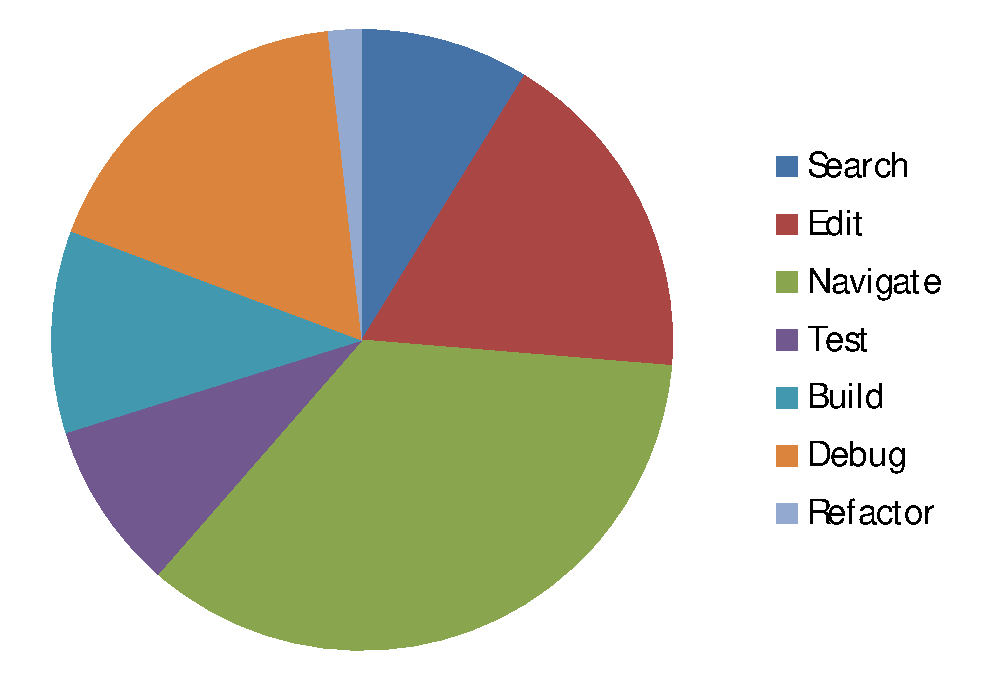
\includegraphics[width=0.5\columnwidth]{../Graphics/activityCategorization.pdf}
%\caption{Pairwise matches across categories, including matching and mismatching pairs.}
%\label{fig:category}
%\end{figure*}
